% reddit-reliability

% http://www.acm.org/publications/article-templates/proceedings-template.html
\documentclass{acm_proc_article-sp}

\usepackage{cleveref} % Better References
\usepackage{lipsum}

\begin{document}

\title{Analysis of Redditor Reliability}

\numberofauthors{1}
\author{
\alignauthor
Kashev Dalmia$^1$, Ryan Freedman$^1$, and Terence Nip$^1$, \\
\texttt{\{dalmia3, rtfreed2, nip2\}@illinois.edu}
\and \and
$^1$University of Illinois at Urbana-Champaign
}


\maketitle
\begin{abstract}
In this paper, we present a system by which to evaluate the reliability of the
users of the popular social network \reddit{}. In the past, \reddit{} has had
numerous identity issues. However, through the efforts of both \reddit{} and the
userbase itself, it is becoming a place where users come to read and discuss
news. Thus, there is a growing need to evaluate the reliability of the suppliers
of information on \reddit{}. We first collect features of both reliable and
unreliable users based on their contributions, and most importantly, the
reaction of the community to their contributions. We then use machine learning
techniques to train a regression model to assign a reliability score to an
arbitrary reddit user.

\end{abstract}

\section{Introduction}
\label{sec:introduction}
<<<<<<< HEAD
\reddit{}, the self-proclaimed `frontpage of the internet`, is slowly becoming
just that; many popular news sources, such as The New York Times and CNN, have
begun to use \reddit{} as a primary source of information in an effort to
leverage the power of the large numbers of users which gather and try to provide
and cross-validate information others have gathered.

In most cases, the information gathered is rather inoccuous. For example, a
subset of \reddit{} users (or \textit{redditors}) gather information from
popular news site and aggregate them on individual, topic-based forums (called
\textit{subreddits}) like \texttt{r/news} or \texttt{r/worldnews}, subreddits
for current events within the United States and the world, respectively.

However, \reddit{}'s track record is not necessarily completely spotless when it
comes to dispersing correct, cross-validated information. For example, during
the Boston bombings of the Boston Marathon in April of 2013, \reddit{} falsely
accused individuals of having been part of the bombings simply because of
circumstantial evidence. Many news sites, including CNN, picked up the story and
publicized it. However, it turned out that the individuals \reddit{} picked out
were completely innocent and were only identified as being potentially involved
because of circumstantial evidence (such as having been missing for long periods
of time).\cite{Potts:2013:IRC:2507065.2507079}.

\reddit{} is also noteworthy for allowing users to \textit{upvote} or
\textit{downvote} user-submitted content, indicating either agreement/interest
or disagreement/disinterest, respectively, with the material at hand. As a side
effect of this, users ultimately promote material that they find to be
interesting to them, and hide material that they find to be out of scope,
irrelevant, or simply not interesting with respect to the subreddit they're in.\cite{Gilbert:2013:WUR:2441776.2441866}


\section{Related Work}
\label{sec:related_work}
Various groups have leveraged social media in the past as a resource for
information retrieval. One group at the University of Illinois at
Urbana-Champaign created a tool called Apollo to do fact finding on Twitter.
Part of their analysis involved gathering credibility for claims and
sources.\cite{Le:2011:DDL:2070942.2071018} This method proved to be critical for
them and could be extended for use in a more community-based environment.

% Another analysis of user behavior on Twitter observed how the silent majority
% of users behaved and attempted to extract information from them.
% \cite{DBLP:journals/corr/TagarelliI15}

Though few in number, there are some groups that have done research on
\reddit{}. An analysis of the behavior of \reddit{} relative to other websites
during the Boston marathon bombings encouraged the idea that, while the actions
taken by one community (\texttt{/r/findbostonbombers}) were destructive,
\reddit{} operates differently than indicated by these events.
\cite{Potts:2013:IRC:2507065.2507079}

Another paper, focused on the analysis of one subreddit (\texttt{/r/sandy}),
finds that ``perspective-created'' content on ``social news sites'' tends to
place above professional content such as reports from CNN.
\cite{Leavitt:2014:UHS:2556288.2557140} This is indicative that ``fresh''
information that would not be otherwise available is present on \reddit{} and
needs retrieval.

Another paper on voting behaviors was done to analyze the underprovision, or
lack of voting participation, on \reddit{}. A surprising statistic to come out
of this was that nearly 52\% of popular links were ignored the first time they
were introduced.\cite{Gilbert:2013:WUR:2441776.2441866} This possibly indicates a
lack of alacrity in terms of information delivery. It is apparent that finding
and detecting information is an important and non-trivial task.


\section{Design}
\label{sec:design}
In this section, we show the design of our system. Additionally, we discuss some
of the challenges, limitations, and design decisions that went into making it.
Finally, we discuss some of the details of the implementation.

\subsection{Gathering Reddit User Names} % (fold)
\label{sub:gathering_reddit_user_names}

The first limitation of the Reddit API is that user names are an `open secret'.
If one has the user name of an account, public information about that account
can be retrieved, but there is no way to directly get user names. Instead, what
we were forced to do was scrape the posts of popular Subreddits and get the user
names of the author of every post and comment. In doing so, we were able to
collect over 150K user names. Of the user names we collected, we randomly
selected around 2K to fully gather data on and run our regression model on.
\\
One issue with this approach is that this makes it impossible to identify non-
participants. If a user never comments on a post, or posts a post themselves,
there is no way to know that that user exists. This is unfortunately an
insurmountable limitation. Instead, we chose only to find good and bad users to
train our classifier, and ignore non-participants.

% subsection gathering_reddit_user_names (end)

\subsection{Reddit API Limits} % (fold)
\label{sub:reddit_api_limits}

Reddit has an API limit of 30 requests per minute. We discovered this limit is
not strictly enforced, but in order to be good citizens and as to not get our
access revoked, we knew we had to design around this constraint. In order to
speed up our ability to access user data (as well as change the features that we
used; see \Cref{sub:picking_user_features}, we crawled user data and put the
raw, unmodified data into a MongoDB instance. This MongoDB served as a cache for
the system. Not were we able to store raw data from Reddit API calls, we were
also able to cache results from more computationally intensive features.

% subsection reddit_api_limits (end)

\subsection{Establishing A Ground Truth} % (fold)
\label{sub:establishing_a_ground_truth}
% will add more detail later. take a look at it, i wrote this at 2 am.
Establishing ground truth was done in two stages. The first stage was to find
reliable users. Finding these users was trivial as the site rewards positive behavior
through karma, which leads to increased visibility. From there the users could
be filtered by their level of contribution manually. Moderators from various
communities were also taken for their work in helping the community. These users
were used in our training set for a +1 reliability score. \\
The second stage was to find users who were unreliable or detrimental to the community.
Eventually, we discovered subreddits dedicated to weeding out users that didn't
contribute and various posts that detailed accounts that were used to abuse the
community. These were used as our training set for a -1 reliability score.

% subsection establishing_a_ground_truth (end)

\subsection{Picking User Features: Exploratory Data Analysis} % (fold)
\label{sub:picking_user_features}

\[ TODO \]

% subsection picking_user_features (end)

\begin{table}[tb]
    \caption{The features used to create the regression model}
    \label{tab:tablename}
    \centering
    \scriptsize

    \begin{tabular}{l|l}
    \hline

    \hline
    \textbf{Feature Description} & \textbf{Importance \%} \\
    \hline
Is Reddit Gold                               & 0.13141645  \\
Has Verified Email                           & 0.75193818  \\
Time Account Created                         & 0.36501668  \\
Flesch--Kincaid Readability of Comments      & 0.1780538   \\
Link Karma                                   & 51.24893713 \\
Number of Gilded Posts                       & 0.          \\
Number of Total Posts                        & 9.34206046  \\
Average Karma per Post                       & 13.51664424 \\
\% of Posts Gilded                           & 0.          \\
Comment Karma                                & 21.0226671  \\
Number of Gilded Comments                    & 0.          \\
Average Comment Karma per Comment            & 0.49150516  \\
\% of Comments Gilded                        & 0.          \\
\% of Post Karma - Trusted Subreddits        & 0.04919857  \\
\% of Post Karma - Top 100 Subreddits        & 0.11182328  \\
\% of Post Karma - Top 50 Subreddits         & 0.10522454  \\
\% of Post Karma - Top 25 Subreddits         & 0.03107503  \\
\% of Post Karma - Top 10 Subreddits         & 0.02660348  \\
\% of Comment Karma - Trusted Subreddits     & 0.11130672  \\
\% of Comment Karma - Top 100 Subreddits     & 1.7193966   \\
\% of Comment Karma - Top 50 Subreddits      & 0.09484735  \\
\% of Comment Karma - Top 25 Subreddits      & 0.06505774  \\
\% of Comment Karma - Top 10 Subreddits      & 0.34236058  \\
\% of Swear Words Used in Comments           & 0.03435242  \\
Unique Words / Total Number Words            & 0.26051451  \\
    \hline

    \hline
    \end{tabular}
\end{table}


\subsection{Picking a Regression Model} % (fold)
\label{sub:picking_a_regression_model}

Something something neural nets give no insight

something something decision trees

something something random forest

something something darkside

% subsection picking_a_regression_model (end)


\section{Evaluation And Results}
\label{sec:evaluation}
From our trained random forest regression model, we get a picture of the way
that redditors are. We get a glimpse of what useful, contributing redditors look
like, and what bad, non-contributing redditors look like.

We collected data on around two thousand redditors, and ran their data through
our regressive model to get a reliability score $-1 \leq s_r \leq 1$. Then, we
re-correlate this score with input features to intuitively see what features are
important or not, and what features indicated useful and not-useful redditors.

\[ TODO \]

\begin{figure}[tb]
    \centering
    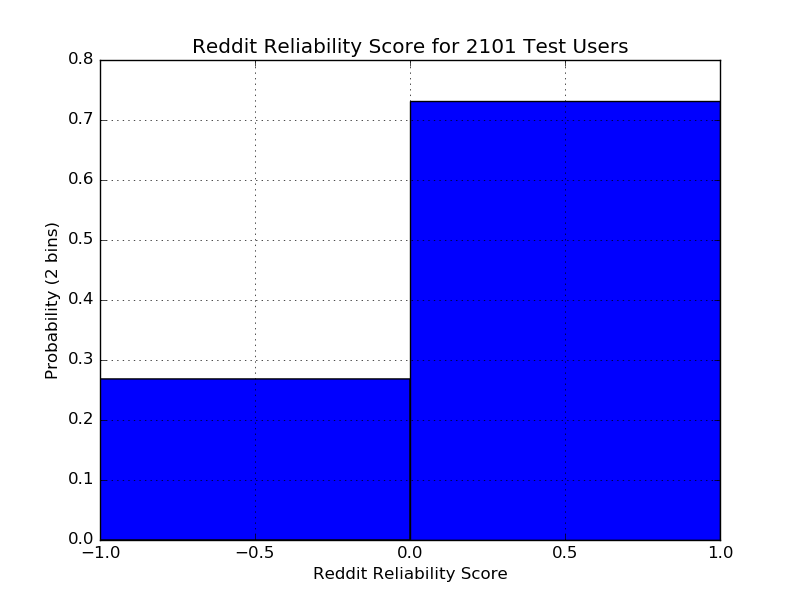
\includegraphics[width=\linewidth]{figures/data_2.png}
    \caption{The distribution of the reliability score $s_r$ of the sampled redditors, binned into two bins.}
    \label{fig:data_2}
\end{figure}

\begin{figure}[tb]
    \centering
    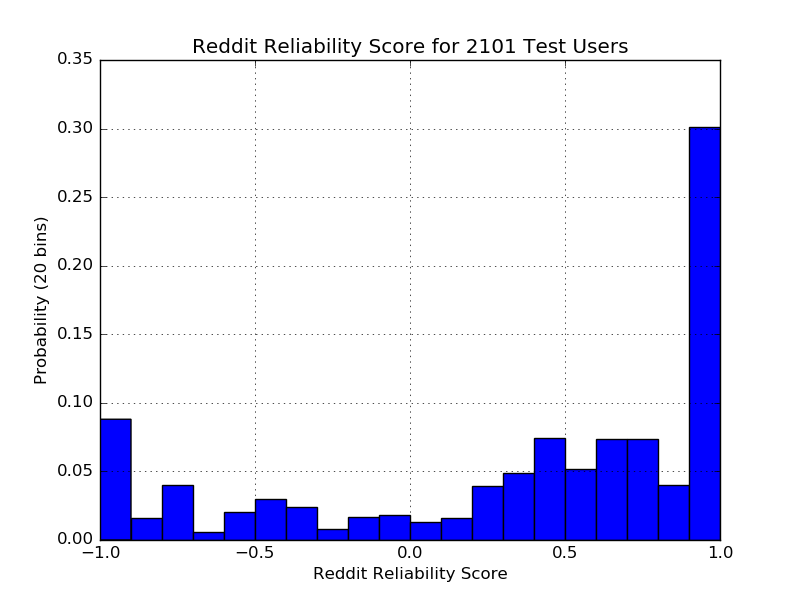
\includegraphics[width=\linewidth]{figures/data_20.png}
    \caption{The distribution of the reliability score $s_r$ of the sampled redditors, binned into twenty bins.}
    \label{fig:data_20}
\end{figure}

\begin{figure}[tb]
    \centering
    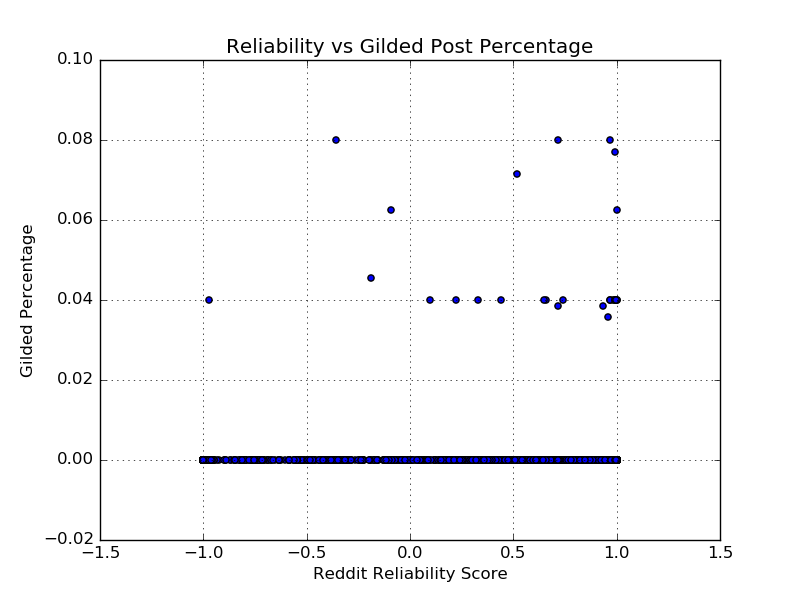
\includegraphics[width=\linewidth]{figures/reliability_gilded.png}
    \caption{The reliability score $s_r$ plotted against the percentage of gilded posts.}
    \label{fig:reliability_gilded}
\end{figure}

\begin{figure}[tb]
    \centering
    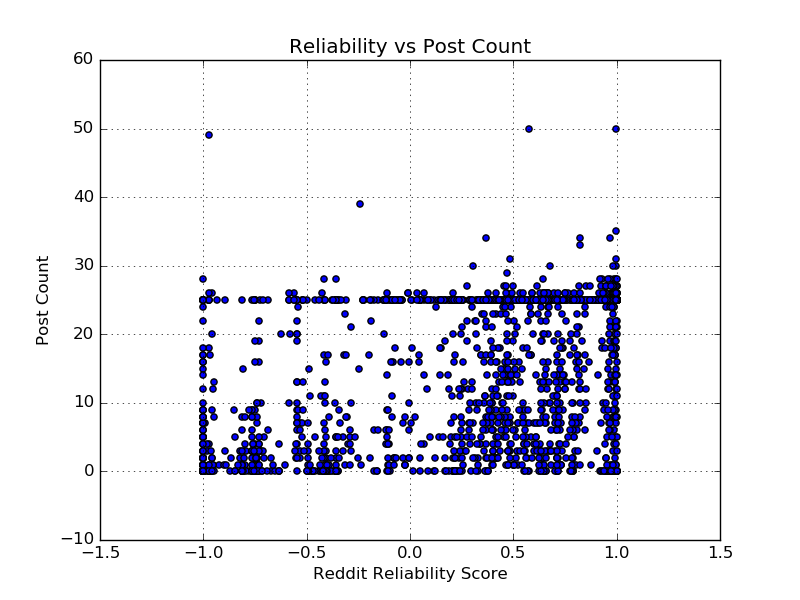
\includegraphics[width=\linewidth]{figures/reliability_post_count.png}
    \caption{The reliability score $s_r$ plotted against the number posts the redditor has made.}
    \label{fig:reliability_post_count}
\end{figure}

\begin{figure}[tb]
    \centering
    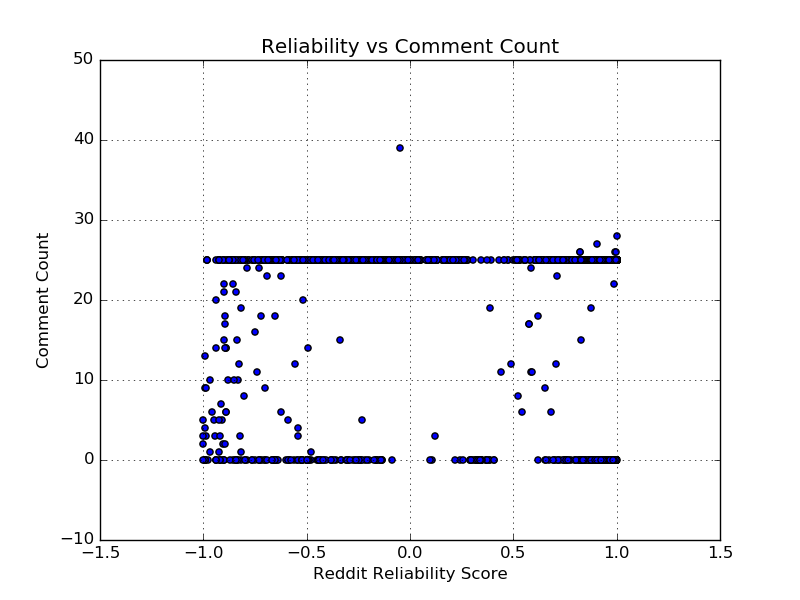
\includegraphics[width=\linewidth]{figures/reliability_comment_count.png}
    \caption{The reliability score $s_r$ plotted against the number posts the redditor has made.}
    \label{fig:reliability_comment_count}
\end{figure}

\begin{figure}[tb]
    \centering
    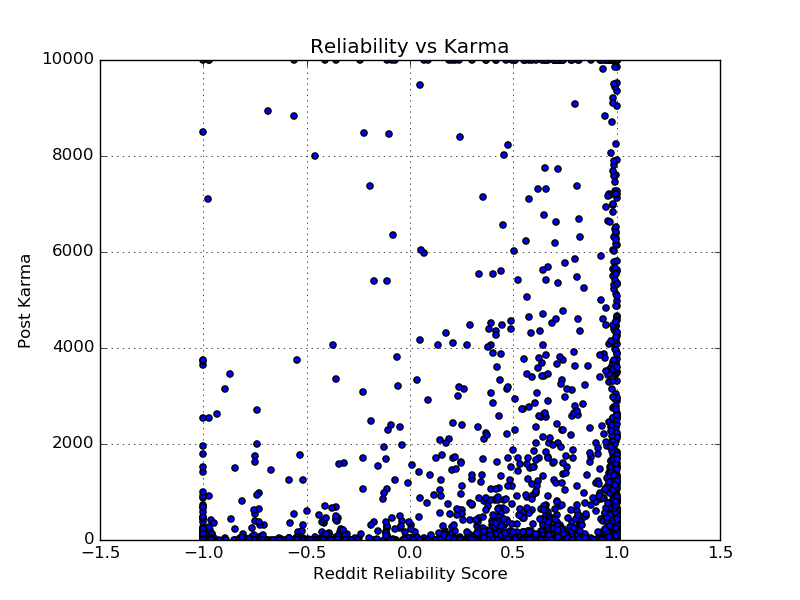
\includegraphics[width=\linewidth]{figures/reliability_post_karma.png}
    \caption{The reliability score $s_r$ plotted against the average Karma per post the redditor has made.}
    \label{fig:reliability_post_karma}
\end{figure}

\begin{figure}[tb]
    \centering
    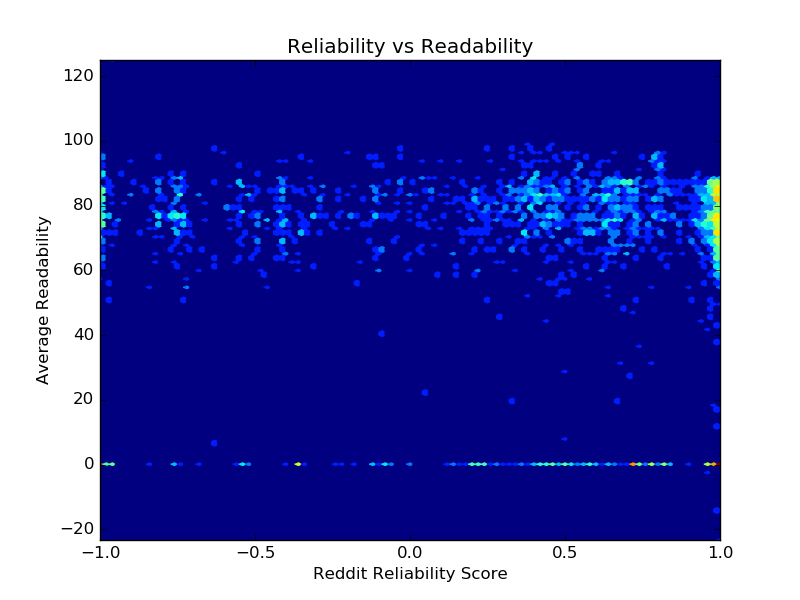
\includegraphics[width=\linewidth]{figures/reliability_readability.png}
    \caption{The reliability score $s_r$ plotted against the Flesch--Kincaid readability of their comments.}
    \label{fig:reliability_readability}
\end{figure}

\begin{figure}[tb]
    \centering
    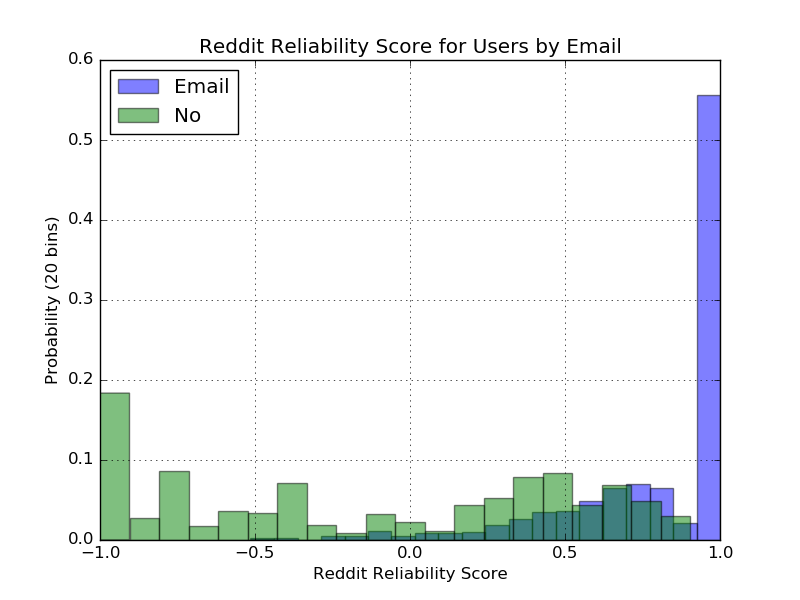
\includegraphics[width=\linewidth]{figures/data_20_email.png}
    \caption{The distribution of the reliability score $s_r$ of the sampled redditors, binned into twenty bins, separated by if they have a verified email address or not.}
    \label{fig:data_20_email}
\end{figure}


\section{Conclusion}
\label{sec:conclusion}
\lipsum[1]

\subsection{Future Work} % (fold)
\label{sub:future_work}

Something something number of posts

Something something many weaknesses

Given the set of users we have obtained in conjunction with the variability that exists among the various subsets of reddit users there exists weaknesses in our analysis. However, given the current state of research of reddit and the increasing reliance of individuals on reddit as a source of reliable information our contribution noteworthy for the purpose of exploration with respect to reddit as an up-and-coming source of information.

Something something exploratory/first exploration of field

\[TODO\]

% subsection future_work (end)


\subsection{Open Issues} % (fold)
\label{sub:open_issues}

Something something hard to establish ground truth

Voting on reddit will always be somewhat ambiguous

% subsection open_issues (end)


\section{Acknowledgments}
The authors would like to thank Professor Tarek F. Abdelzaher, of the University
of Illinois at Urbana-Champaign, for his support in this project.

\bibliographystyle{abbrv}
\bibliography{references}

\end{document}
